\documentclass[12pt, letterpaper]{article}

% Imports
\usepackage{fancyhdr}
\usepackage{geometry}
\usepackage{icomma}
\usepackage{amsmath}
\usepackage{multicol}
\usepackage{mathptmx}
\usepackage{anyfontsize}
\usepackage{t1enc}
\usepackage{tabto}
\usepackage{listings}
\usepackage{filecontents}
\usepackage{subcaption}
\usepackage{tikz}
\usepackage[parfill]{parskip}
\usepackage{graphicx}
\usepackage[]{mdframed}
\usepackage{amsmath}
\usepackage[makeroom]{cancel}
\usepackage{pgfplots}
\usepackage{pgfplotstable}
\usepackage{xfrac}
\usepackage{amssymb}
\usepackage{mathtools}
\pgfplotsset{compat=1.18}
\usetikzlibrary{patterns}
\usepgfplotslibrary{polar}
\usepgfplotslibrary{fillbetween}

\geometry{margin=2.5cm}

\newcommand{\name}{Kaleb Burris}
\newcommand{\classname}{MATH F253, Elizabeth S. Allman, University of Alaska Fairbanks}
\newcommand{\assignment}{FILL IN ASSIGNMENT NAME}

\pagestyle{fancy}

\fancyhead[L]{
    \name 
    \newline
    \classname
    \newline
    \assignment
}

\newcommand{\horizontal}{\noindent\rule{\hsize}{0.4pt}}

\setlength{\headheight}{42pt}
\setlength{\headsep}{0.25in}
\setlength{\columnsep}{0.35cm}
\setlength{\columnseprule}{1pt}

\usepackage[T1]{fontenc}
\usepackage{lmodern}

% Put class number, class name, and professor 
% name.
% Use only in case of emergency, this
% should be covered by the preamble.
% \renewcommand\classname{}

% Put the assignment name with \S if 
% necessary for the section and the question 
% numbers.
\renewcommand\assignment{Lab 1: Uncertainty Analysis, 9/7/2023, Partner: Quency Snow}

\graphicspath{ {./lab01images/} }

\begin{document}
    \section*{Part 1: Propagation of Uncertainty}
    \begin{enumerate}
        \item[1.] Refer to Equation 5, differentiate to find the equation for $\delta x$.
        
        \begin{mdframed}
            \begin{equation*}
                x = 2M_{p+b}m_{b}^{-1}y^{\frac{1}{2}}\Delta h^{\frac{1}{2}} \quad (5)
            \end{equation*}

            \begin{equation*}
                \begin{gathered}
                    \delta x = \sqrt{
                        \left(\frac{\partial x}{\partial M_{p+b}}\delta M_{p+b}\right)^{2} + 
                        \left(\frac{\partial x}{\partial m_{b}}\delta m_{b}\right)^{2} + 
                        \left(\frac{\partial x}{\partial y}\delta y\right)^{2} + 
                        \left(\frac{\partial x}{\partial \Delta h}\delta \Delta h\right)^{2}
                    }\\
                    \frac{\partial x}{\partial M_{p+b}} = 2m_{b}y^{\frac{1}{2}}\Delta h^{\frac{1}{2}} \\
                    \frac{\partial x}{\partial m_{b}} = 2M_{p+b}y^{\frac{1}{2}}\Delta h^{\frac{1}{2}} \\
                    \frac{\partial x}{\partial y} = M_{p+b}m_{b}^{-1}y^{-\frac{1}{2}}\Delta h^{\frac{1}{2}} \\
                    \frac{\partial x}{\partial \Delta h} = M_{p+b}m_{b}^{-1}y^{-\frac{1}{2}}\Delta h^{-\frac{1}{2}} \\
                    \boxed{\delta x = \sqrt{\begin{lgathered}
                        \left(2m_{b}y^{\frac{1}{2}}\Delta h^{\frac{1}{2}}\delta M_{p+b}\right)^{2} + 
                        \left(2M_{p+b}y^{\frac{1}{2}}\Delta h^{\frac{1}{2}}\delta m_{b}\right)^{2} \\ +
                        \left(M_{p+b}m_{b}^{-1}y^{-\frac{1}{2}}\Delta h^{\frac{1}{2}}\delta y\right)^{2} + 
                        \left(M_{p+b}m_{b}^{-1}y^{-\frac{1}{2}}\Delta h^{-\frac{1}{2}}\delta \Delta h\right)^{2}
                    \end{lgathered}}}
                \end{gathered}
            \end{equation*}
        \end{mdframed}

        \item[2.] Differentiate to find the equation to propagate the uncertainty $\delta L$.
        
        \begin{mdframed}
            \begin{equation*}
                \begin{gathered}
                    L_{f} = m_{ice}^{-1}(c_{w}m_{h}+C_{d})(T_{h}-T_{f})+c_{w}(T_{ice}-T_{f}) \\\
                    \delta c_{W} = 0    \\
                    \frac{\partial L}{\partial m_{ice}} = -m_{ice}^{-2}(c_{w}m_{h}+C_{d})(T_{h}-T_{f}) \\
                    \frac{\partial L}{\partial m_{h}} = m_{ice}^{-1}(c_{w}T_{ice} - c_{w}T_{f}) \\
                    \frac{\partial L}{\partial C_{d}} = m_{ice}^{-1}(c_{d}T_{ice} - C_{d}T_{f}) \\
                    \frac{\partial L}{\partial T_{ice}} = c_{w} \\
                    \frac{\partial L}{\partial T_{f}} = -c_{w}  \\
                    \boxed{\delta L = \sqrt{ \begin{lgathered}
                        \left(-m_{ice}^{-2}(c_{w}m_{h}+C_{d})(T_{h}-T_{f})\delta m_{ice}\right)^{2} +
                        \left(m_{ice}^{-1}(c_{w}T_{ice} - c_{w}T_{f})\delta m_{h}\right)^{2} \\ +
                        \left(m_{ice}^{-1}(c_{d}T_{ice} - C_{d}T_{f})\delta C_{d}\right)^{2} +
                        \left(c_{w}\delta T_{ice}\right)^{2} +
                        \left(-c_{w}\delta T_{f}\right)^{2}
                    \end{lgathered}}} \\
                \end{gathered}
            \end{equation*}
        \end{mdframed}

    \end{enumerate}

    \section*{Part 2: Caliper}

    \begin{enumerate}
        \item [3.] Measure the outer dimensions of the 1-2-3 Block with the calipers in cm.
        
        \begin{mdframed}
            \begin{center}
                \begin{tabular}{|c|c|}
                    \hline
                    3-side & 7.3cm $\pm$ 0.05cm \\
                    \hline
                    2-side & 4.8cm $\pm$ 0.05cm \\
                    \hline
                    1-side & 2.2cm $\pm$ 0.05cm \\
                    \hline
                \end{tabular}    
            \end{center}
        \end{mdframed}

        \item [4.] Convert your measurements and uncertainties to inches, then compare your values to the accepted values of the outer dimensions of the 1-2-3 block.
        
        \begin{mdframed}
            3-Side: 2.87in $\pm$ 0.02in; not within accepted value of 3in.
            2-Side: 1.89in $\pm$ 0.02in; not within accepted value of 2in.
            1-Side: 0.87in $\pm$ 0.02in; not within accepted value of 1in.
        \end{mdframed}
    \end{enumerate}    


    \section*{Part 3: DMM}

    \begin{enumerate}
        \item [5.] Measure the voltage of the batteries. Compare to the accepted value.
        
        \begin{mdframed}
            \begin{tabular}{|c|c|p{3in}|}
                \hline
                Measured Voltage & Accepted Value & Comparison  \\
                \hline
                1.562V $\pm$ 0.0005V & 1.5V & Within accepted voltage.  \\
                \hline
                3.30V $\pm$ 0.005V & 6V & Significantly off of accepted voltage; \ the battery is probably in need of replacement. \\
                \hline
            \end{tabular}
        \end{mdframed}

        \item[6.] Measure each of the resistors. Refer to Figure 6. What is the color code value and tolerance for each of your resistors? Are your measurements within the tolerance of each resistor?
        
        \begin{mdframed}
            \begin{center}
                \begin{tabular}{|c|c|c|c|}
                    \hline
                    Resistor Color Code & Measured Resistance & Accepted Resistance & Tolerance \\
                    \hline
                    OOOS & 33.1K $\Omega\; \pm$ 0.01K $\Omega$ & 33.0K $\Omega$ & $\pm$10\%     \\
                    \hline
                    bBYS & 101.2K $\Omega\; \pm$ 0.01K $\Omega$ & 100.0K $\Omega$ & $\pm$10\%   \\
                    \hline
                \end{tabular}    
            \end{center}
        \end{mdframed}

        \item[7.] Compare your values to the accepted values.
        
        \begin{mdframed}
            All of our measured resistances were well within the accepted tolerance range of 10\%, that being: (34.0 $\geq$ 33.1 $\geq$ 32.0) and (110.0 $\geq$ 101.2 $\geq$ 90.0).
        \end{mdframed}
    \end{enumerate}

    \section*{Part 4: LoggerPro Review and Uncertainty Application}
    \begin{enumerate}
        \item [8.] Measure the mass of the basketball. Report the mass and its uncertainty as $m \pm \delta m$.
        
        \begin{mdframed}
            Mass = 599.6g ± 0.5 g = 0.599kg ± 0.0005kg
        \end{mdframed}

        \pagebreak

        \item[9.] Analyze the first three positive slopes of the velocity vs. time graph.
        
        \begin{itemize}
            \item [a., b.]\mbox{}
            
            \begin{mdframed}
                \begin{center}
                    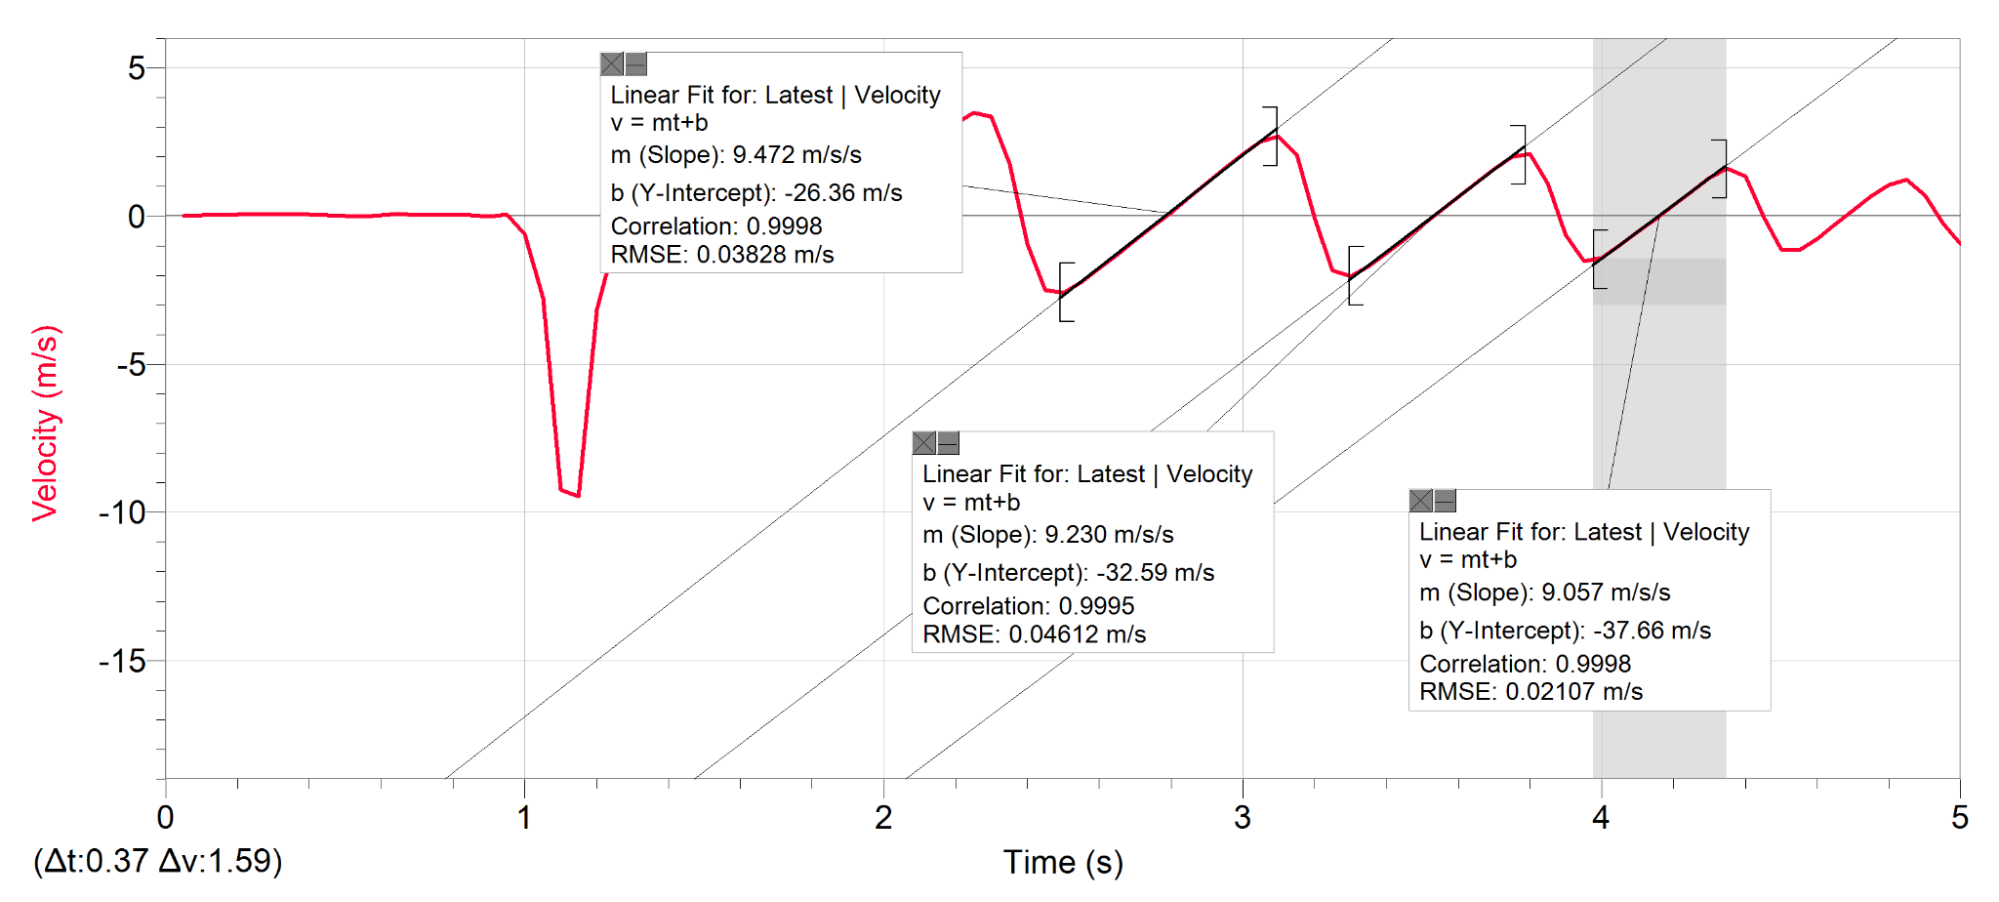
\includegraphics[width=\textwidth]{image3.png}
                \end{center}
            \end{mdframed}

            \item[c.] Compare to $g = 9.80m/s^{2}$ by calculating the percent error for each.
            
            \begin{mdframed}
                \begin{align*}
                    E_{1} & = \frac{|9.80 - 9.472|}{\frac{9.80 + 9.472}{2}}  \time 100
                            = \frac{0.33}{9.63} \times 100 = 3.43 \%    \\
                    E_{2} & = \frac{|9.80 - 9.230|}{\frac{9.80 + 9.230}{2}}  \time 100
                            = \frac{0.57}{9.52} \times 100 = 5.99 \%    \\
                    E_{3} & = \frac{|9.80 - 9.057|}{\frac{9.80 + 9.057}{2}}  \time 100
                            = \frac{0.74}{9.43} \times 100 = 7.85 \%    \\
                \end{align*}

                The error found here is within 10\%, and gradually increases with each bounce. 
                
                This could be due to a torque induced onto the ball when it's been dropped and/or a torque induced when it makes contact with the ground. 
                
                There are also energy losses to the ground that make the ball's velocity decrease and thus decrease the amount of data recorded for a bounce. 
                
                The range selected for the linear fits also has some variance that could affect the error (although they appear to be selected very accurately).
            \end{mdframed}
        \end{itemize}

        \pagebreak

        \item[10.] We will need to determine the velocity and its uncertainty uncertainty ($v \pm \delta v$) from the position vs. time graph. To determine the uncertainty of a measurement from Logger Pro we will need to do a line of best fit.
        
        \begin{itemize}

            \item [a., b., c., e.]\mbox{}
            
            \begin{mdframed}
                \begin{center}
                    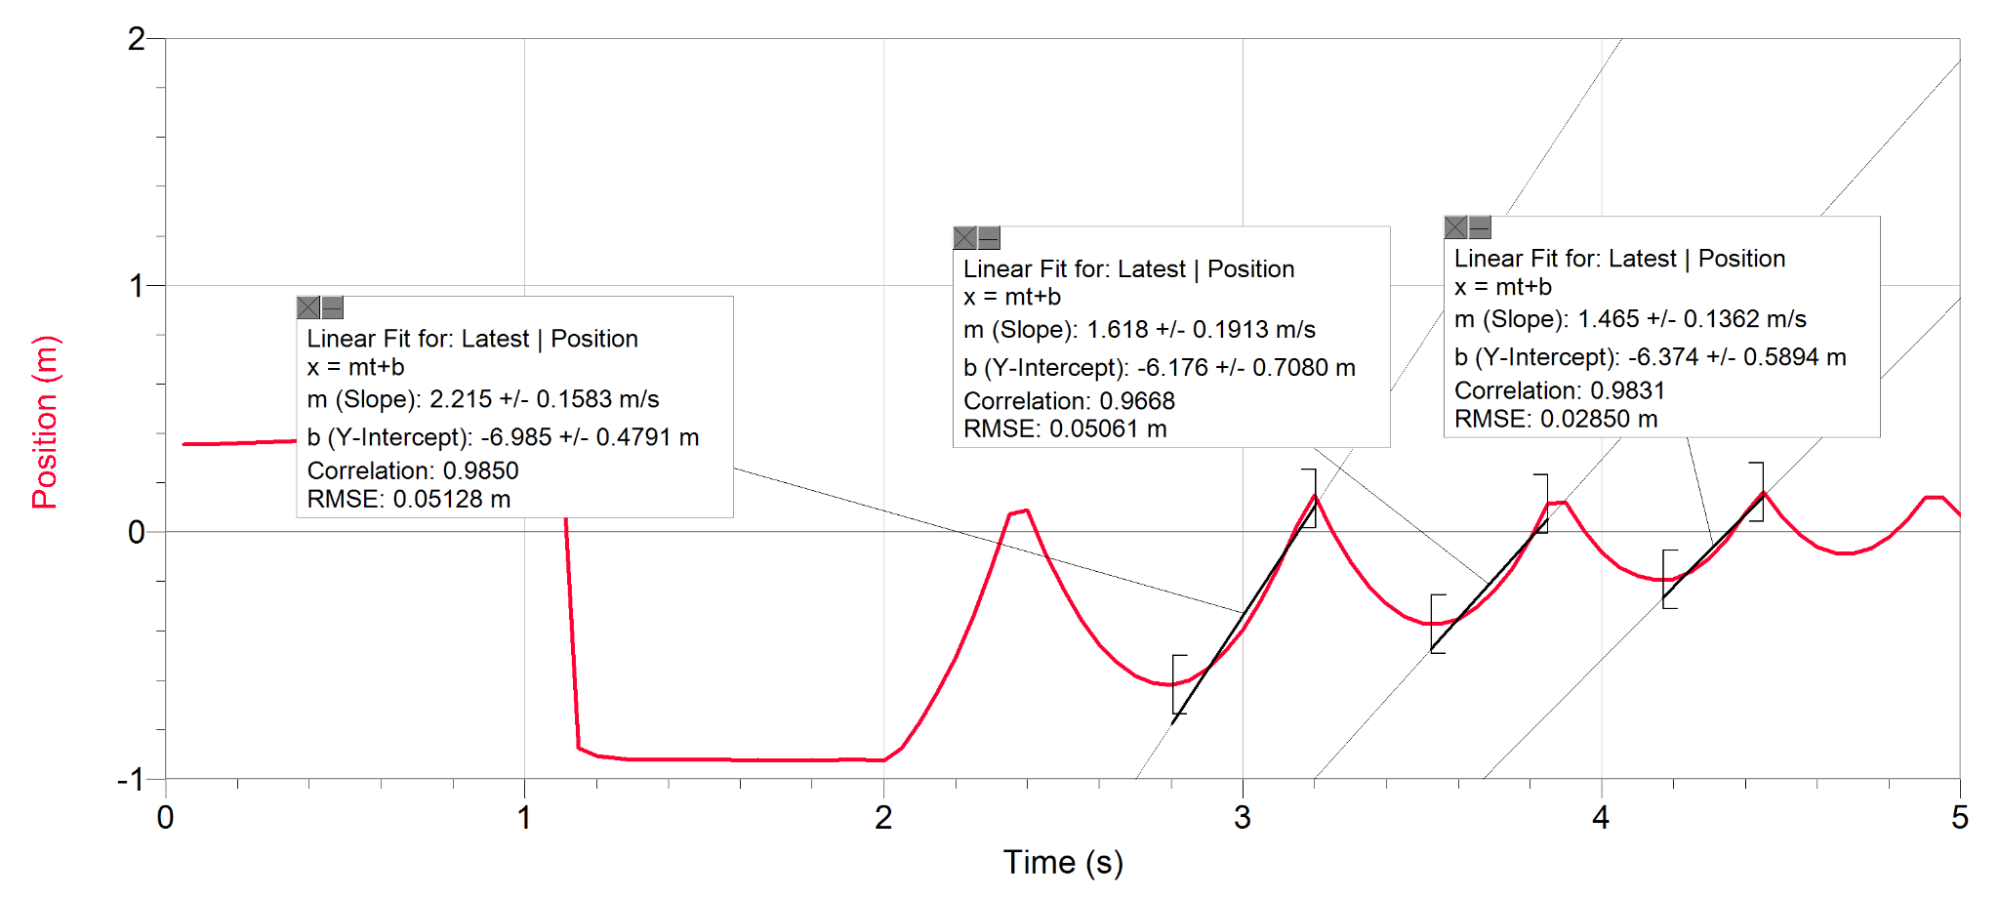
\includegraphics[width=\textwidth]{image5.png}

                    \boxed{2.215 m/s \pm 0.1583 m/s}
                \end{center}
            \end{mdframed}
        \end{itemize}

        \item[11.] Create a calculated column for kinetic energy and graph it.
        
        \begin{mdframed}
            \begin{center}
                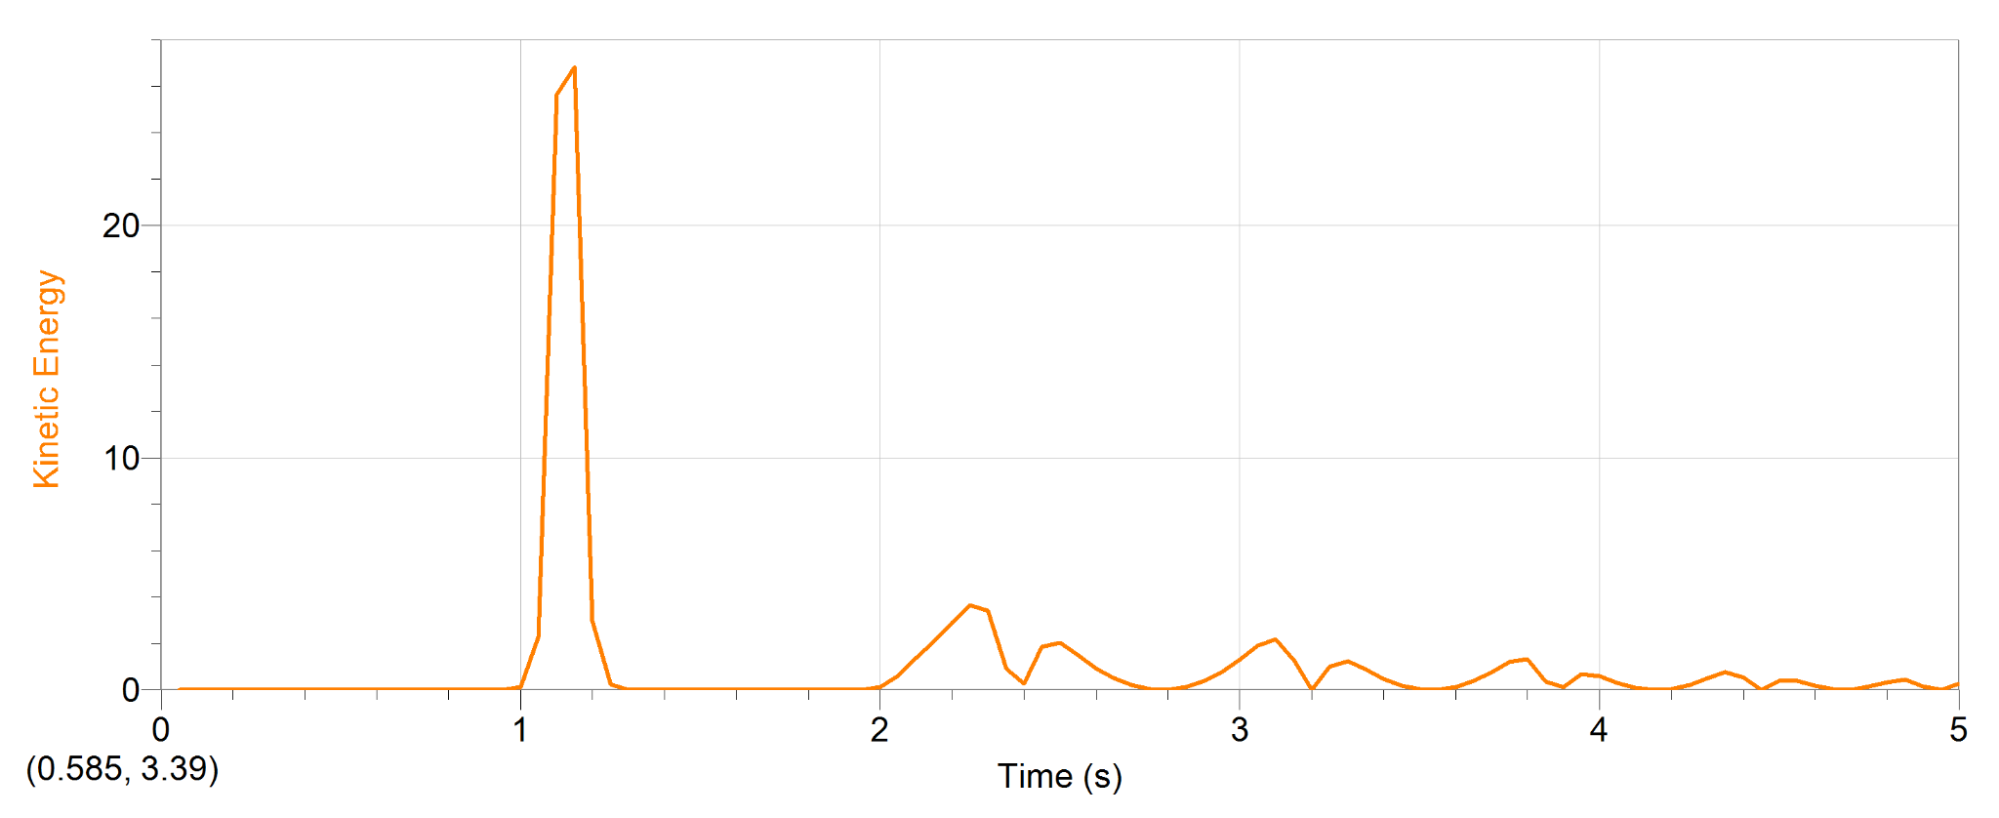
\includegraphics[width=\textwidth]{image1.png}
            \end{center}
        \end{mdframed}
    \end{enumerate}
\end{document}